\appendix


\chapter{Datasheets and Plots}
\section{Kinetic parameter normal distribution}

\begin{table}
    \caption[Mean and covariance of the parameters]{
        Mean and covariance matrix of the activation energies and pre-exponential collision factors.
        }
        \begin{tabular}{l r | r r r r}
            \toprule
            \multicolumn{2}{c|}{$\boldsymbol{\mu}$} & \multicolumn{4}{c}{$\boldsymbol{\Sigma}$} \\ 
            \cmidrule(lr){3-6}
            \multicolumn{1}{c}{} & \multicolumn{1}{c|}{} & 
            \multicolumn{1}{c}{$\ln k_{0,1}$} & 
            \multicolumn{1}{c}{$E_{\text{A},1}$} & 
            \multicolumn{1}{c}{$\ln k_{0,2}$} & 
            \multicolumn{1}{c}{$E_{\text{A},2}$} \\
            \midrule
            $\ln k_{0,1}$ & 15.621453 & 0.351544 & 1768.109910 & 0.380453 & 1913.304578 \\
            $E_{\text{A},1}$ & 74856.339000 & 1768.109910 & 9031744.980000 & 1913.445056 & 9773020.700000 \\
            $\ln k_{0,2}$ & 16.272557 & 0.380453 & 1913.445056 & 0.411795 & 2070.851800 \\
            $E_{\text{A},2}$ & 89853.839400 & 1913.304578 & 9773020.700000 & 2070.851800 & 10576522.400000 \\
            \bottomrule
        \end{tabular}
    \label{app:tab:mean-and-covariance}
\end{table}


\section{Temperature Trajectories}
\begin{figure}
    \centering
    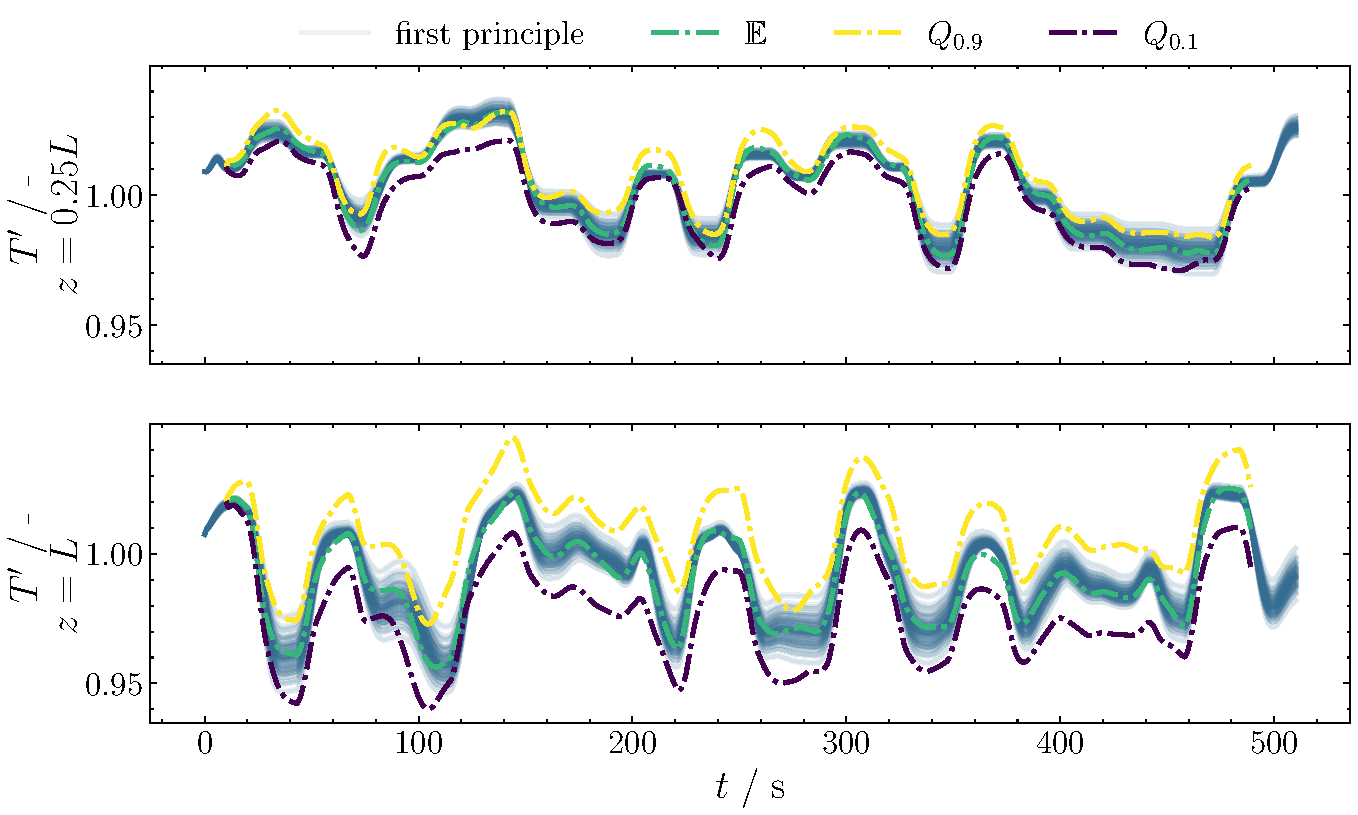
\includegraphics[width=1\textwidth]{Figures/Results/test_with_naive_pc_-1.pdf}
    \caption[Forward simulation of the naive NARX framework for the temperature quantiles.]
    {Forward simulation of the NARX framework with the constrained activation applied a posteriori for 
    \SI{480}{\second}.}
    \label{app:fig:naive-temperature-sim}
\end{figure}
\begin{figure}
    \centering
    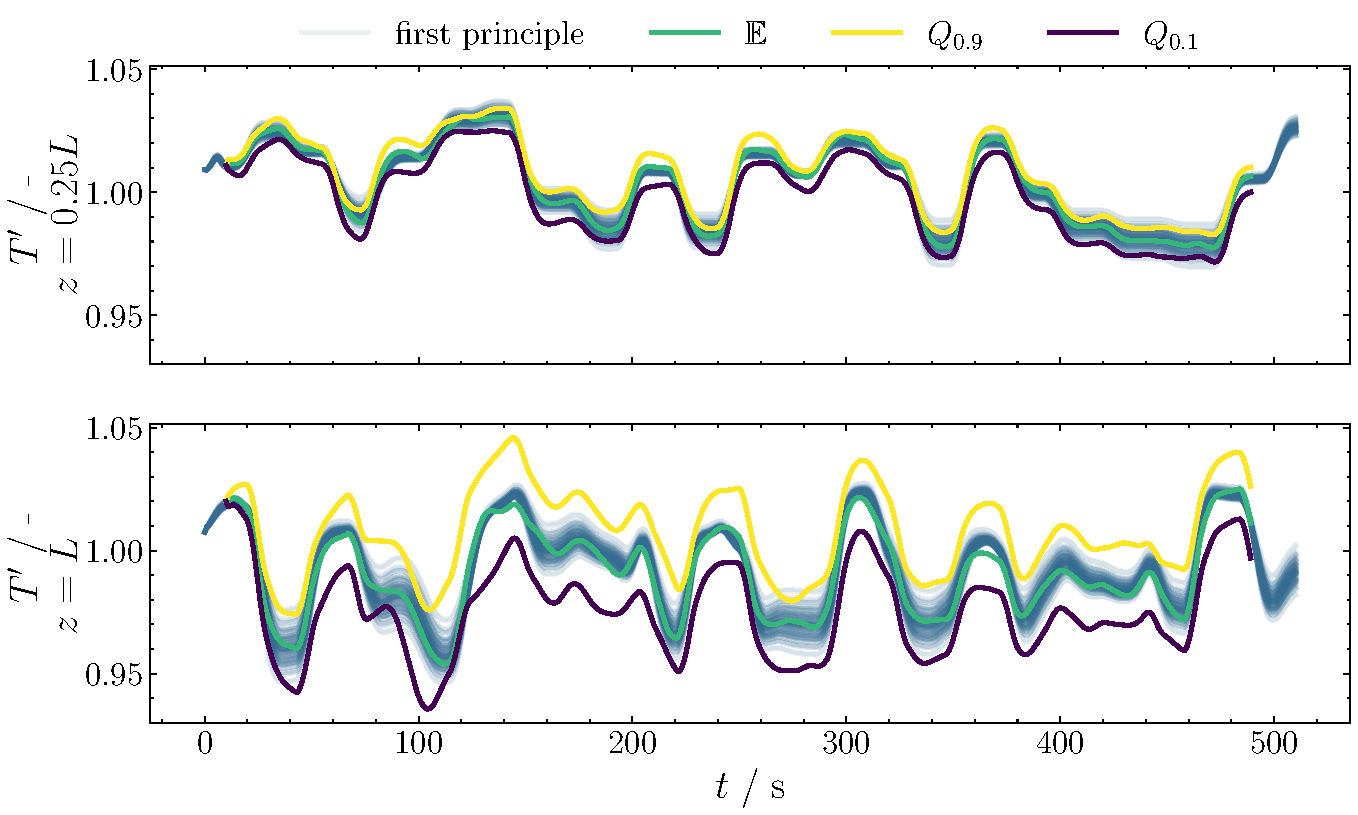
\includegraphics[width=1\textwidth]{Figures/Results/test_with_pc_-1.pdf}
    \caption[Forward simulation of the pc NARX framework for the temperature quantiles.]
    {Forward simulation of the NARX framework with the constrained activation applied during training and simulation
    for \SI{480}{\second}.}
    \label{app:fig:pc-temperature-sim}
\end{figure}

\chapter{Proofs and Code}
\section{Code}

\subsection{Inverse calculation and forward method to apply the pc activation}
\label{app:code:forward-pass}
\begin{lstlisting}[frame=single]
def set_linear_equality_constraint(self, A: torch.Tensor, b: torch.Tensor = None):
    b = b or torch.zeros(A.shape[0], dtype=A.dtype)
    U = torch.cat([2 * torch.eye(A.shape[1], dtype=A.dtype, device=A.device), A.T], dim=1)
    L = torch.cat([A, torch.zeros((A.shape[0], A.shape[0]), dtype=A.dtype, device=A.device)], dim=1)
    projection_inverse = torch.linalg.inv(torch.cat([U, L], dim=0))
    ru_vec = self.boundary_cond @ A.T + b

    self.register_buffer("projection_inverse", projection_inverse)
    self.register_buffer("constraint_matrix", A)
    self.register_buffer("constraint_rhs", b)
    self.register_buffer("ru_vec", ru_vec)

def forward(self, x: torch.Tensor) -> torch.Tensor:
    x = super().forward(x)
    ru = torch.repeat_interleave(self.ru_vec, repeats=x.shape[0], dim=0)  # repeat to allow batching
    intermediate_vector = torch.cat([2 * x, ru], dim=-1)
    x = intermediate_vector @ self.projection_inverse
    x = x[..., : self.n_output]  # cutting dual variables
    # no output scaler
    return x
\end{lstlisting}


\section{Model Derivation}

\subsection{Component Mass Balance in local form}
\begin{equation}
    \label{app:eq:component-mass-balance}
    \begin{aligned}
        \frac{\partial \rho_{\alpha}}{\partial t} &=
        -\frac{\partial}{\partial z_k} \left( \rho_{\alpha} u_k + j_{k,\alpha} \right)
        + \sigma_{\alpha} \quad \left[ \frac{\text{kg}}{\text{s} \cdot \text{m}_\text{R}^3} \right] \\
        \frac{\partial c_{\alpha}}{\partial t} &= 
        -\frac{\partial}{\partial z} \left( c_{\alpha} u \right) +
        R_\alpha (c_{\alpha}, T) \\
        \frac{\partial c_{\alpha}}{\partial t} &=
         - \frac{\partial}{\partial z} \left( c_{\alpha} u \right) +
         (1-\varepsilon) \sum_{j}^{N_\text{r}} \nu_{\alpha j} \cdot r_j \\
        \frac{\partial}{\partial t} \left( \frac{p x_{\alpha}}{\mathrm{R}T} \right) &= 
        -\frac{\partial}{\partial z} \left( \frac{p x_{\alpha}}{\mathrm{R}T} u \right) +
        (1-\varepsilon) \sum \nu_{\alpha j} \cdot r_{j} \\
        \frac{\partial}{\partial t} \left( \frac{x_{\alpha}}{T} \right) &=
         -\frac{\partial}{\partial z} \left( \frac{x_{\alpha}}{T} u \right) +
         (1-\varepsilon) \frac{\mathrm{R}}{p} \sum \nu_{\alpha j} \cdot r_{j} \\
        \frac{\partial}{\partial t} \left( \frac{x_{\alpha}' x_{\alpha *}}{T' T_*} \right) &= 
        -u \frac{\partial}{\partial z} \left( \frac{x_{\alpha}' x_{\alpha *}}{T' T_*} \right) +
        (1-\varepsilon) \frac{\mathrm{R}}{p} \sum \nu_{\alpha j} \cdot r_j \\
        \frac{\partial}{\partial t} \left( \frac{x_{\alpha}'}{T'} \right) &=
         -u \frac{\partial}{\partial z} \left( \frac{x_{\alpha}'}{T'} \right) +
         (1-\varepsilon) \frac{\mathrm{R} \cdot T_*}{p \cdot x_{\alpha *}}
         \sum \nu_{\alpha j} \cdot r_j (\chi_{\alpha}', T') \\
        \frac{\partial \chi_{\alpha}}{\partial t} &= 
        - u \frac{\partial \chi_{\alpha}}{\partial z} +
        (1-\varepsilon) \frac{\mathrm{R}}{P} \frac{T_*}{x_*}
        + \sum_i \nu_{\alpha j} \cdot r_j (\chi_{\alpha}, T)
    \end{aligned}
\end{equation}

\subsection{Enthalpy Balance in local form}
\begin{equation}
    \label{app:eq:enthalpy-balance}
    \begin{aligned}
        \frac{\partial (\rho h)}{\partial t} - \frac{\partial p }{\partial t} &= 
        -\frac{\partial}{\partial z_k} \bigg (\rho h u_k + q_k' \bigg) + 
        u_k \frac{\partial p}{\partial z_k} + \sum_i j_{k,i} f_{k,i} -
        \Pi_{j,k} \frac{\partial u_j}{\partial z_k} + \sigma_h \\
        \rho \frac{\partial h}{\partial t} - \frac{\partial p}{\partial t} &=
        - \rho u \frac{\partial h}{\partial z} + u \frac{\partial p}{\partial z} + \sigma_h \\
        \rho \frac{\partial h}{\partial t} &= - \rho u \frac{\partial h}{\partial z} + \sigma_h \\
        \rho c_p \frac{\partial T}{\partial t} &= - \rho u c_p \frac{\partial T}{\partial z} + \sigma_h \\
        \frac{\partial T'}{\partial t} &= - u \frac{\partial T'}{\partial z} + \frac{1}{\rho c_p T_*} \sigma_h \\
    \end{aligned}
\end{equation}
\begin{equation}
    \label{app:eq:enthalpy-soruce-term}
    \sigma_h = (1-\epsilon) \sum_j^{N_\text{r}} (-\Delta h_{\text{R},j})r_j
        + \frac{4}{d_\text{t}} \alpha (T_\text{w} - T) 
        \quad \quad \left[ \frac{\si{\joule}}{\si{\second} \cdot \si{\meter}_\text{R}^3} \right]
\end{equation}
\begin{equation}
    \label{app:eq:differential-of-enthalpy}
    \begin{aligned}
        dh &= T ds - v dp \quad \text{with} \quad v = \frac{\text{R}T}{p}
        \quad \text{and} \quad ds = dq/T \\
        dh &= dq - \frac{\text{R}T}{p}dp \quad \quad \Big | \quad dq = c_\text{p}dT \quad \text{and} \quad dp = 0 \\
        dh &= c_\text{p}dT
    \end{aligned}
\end{equation}

\subsection{Lumped Properties}
\begin{equation}
    \label{app:eq:lumped-properties}
    \begin{aligned}
        \rho &= \epsilon \rho_\text{g} + (1-\epsilon) \rho_\text{s} \\
        \rho_\text{g}(T) &= \frac{M_\text{tot} p}{\text{R}T} \\
        c_\text{p} &= \epsilon c_\text{p,g} + (1-\epsilon) c_\text{p,s}
    \end{aligned}
\end{equation}

\subsection{Heat Transfer Correlations}
\begin{equation}
    \label{app:eq:nusselt-number}
    \mathrm{Nu}_\text{w} = \frac{\alpha d_\text{p}}{\lambda_\text{g}}
\end{equation}
\begin{equation}
    \label{app:eq:nusselt-number-VDI}
    \begin{gathered}
        \mathrm{Nu}_\text{w} = \bigg (1.3 + 5 \frac{d_\text{p}}{d_\text{t}} \bigg) \frac{\lambda_\text{bed}}{\lambda_\text{g}}
        + 0.19 \; \mathrm{Re}_0^{3/4} \mathrm{Pr}^{1/3}
        \quad \quad \text{\cite{vdiwaermeatlas2010}} \\
        \text{with} \quad 1.2 < \frac{d_\text{t}}{d_\text{p}} < 51
    \end{gathered}
\end{equation}
\begin{equation}
    \label{app:eq:prandl-number}
    \mathrm{Pr} = \frac{\mu_\text{g} c_\text{p,g}}{\lambda_\text{g} M_\text{tot}}
\end{equation}
\begin{equation}
    \label{app:eq:reynolds-number}
    \mathrm{Re}_0 = \frac{u_0 \rho_\text{g} d_\text{p}}{\mu_\text{g}}
\end{equation}


\begin{equation}
    \label{app:eq:radial-heat-conductivity}
    \lambda_\text{bed} = \lambda_\text{g} (1-(1-\epsilon_0)^{1/2}) + (1-\epsilon_0)^{1/2}k_\text{c}
\end{equation}
\begin{equation}
    \label{app:eq:k-core}
    k_\text{c} = \frac{2}{N} \bigg (\frac{B}{N^2} \frac{\lambda_\text{p} - \lambda_\text{g}}{\lambda_\text{p}}
    \ln \bigg(\frac{k_\text{p}}{B} \bigg) - \frac{B+1}{2} - \frac{B-1}{N}\bigg)
    \quad \quad \text{\cite{zehner1970}}
\end{equation}
\begin{equation}
    \label{app:eq:k-core-auxillary-variables}
    N = 1 + \frac{B \lambda_\text{f}}{\lambda_\text{p}} \quad
    B = 1.25 \bigg (\frac{1-\epsilon_0}{\epsilon_0} \bigg)^{10/9} \quad
    k_\text{p} = \frac{\lambda_\text{p}}{\lambda_\text{g}}
\end{equation}
\begin{equation}
    \label{app:eq:bed-porosity}
    \epsilon = \epsilon_0 + (1-\epsilon_0) \frac{0.526 d_\text{p}}{d_\text{t}}
    \quad \quad \text{\cite{vdiwaermeatlas2010}}
\end{equation}
\begin{equation}
    \label{app:eq:gas-viscosity-function-temperature}
    \mu_\text{g}(T) = A_\mu T^2 + B_\mu T + C_\mu \quad \quad \text{\cite{pietschak2018}}
\end{equation}


\subsection{Change in molar Amount}
\label{app:molar-amount}
\begin{equation}
    \begin{aligned}
        \Delta n_i &= x_{i,0} n_0 - x_i n = x_{i,0} \frac{p_0 V_0}{\mathrm{R} T_0} - x_i \frac{p V}{\mathrm{R} T} \quad | \; \text{isobaric, non-compressible} \\
                &= \bigg ( \frac{x_{i,0}}{T_0} - \frac{x_i}{T} \bigg ) \frac{pV}{\mathrm{R}}
                = \bigg ( \frac{x'_{i,0}}{T'_0} - \frac{x'_i}{T'} \bigg ) \frac{pV}{\mathrm{R}} \frac{x_*}{T_*} \\
                &= ( \chi_{i,0} - \chi_{i} ) \frac{pV}{\mathrm{R}} \frac{x_*}{T_*}
    \end{aligned}
\end{equation}

\newpage
\subsection{Modelling Nomenclature}
\begin{longtable}{@{\extracolsep{\fill}}l l p{7cm}@{}}
    \hline
    \textbf{Symbol} & \textbf{Unit} & \textbf{Description} \\
    \hline
    \multicolumn{3}{l}{\textbf{Latin Symbols}} \\
    $A_\mu, B_\mu, C_\mu$ & \si{\pascal\second\per\kelvin\squared}, \si{\pascal\second\per\kelvin}, \si{\pascal\second}
    & Coefficients for gas viscosity calculation \\
    $B$ & - & Auxiliary parameter for thermal conductivity \\
    $c_{\alpha}$ & \si{\mole\per\cubic\meter} & Molar concentration of component $\alpha$ \\
    $c_p$ & \si{\joule\per\kilogram\per\kelvin} & Specific heat capacity (mixture) \\
    $c_{p,g}$ & \si{\joule\per\kilogram\per\kelvin} & Specific heat capacity of the gas phase \\
    $c_{p,s}$ & \si{\joule\per\kilogram\per\kelvin} & Specific heat capacity of the solid phase \\
    $d_p$ & \si{\meter} & Particle diameter \\
    $d_t$ & \si{\meter} & Tube (reactor) diameter \\
    $h$ & \si{\joule\per\kilogram} & Specific enthalpy \\
    $\Delta h_{\text{R},j}$ & \si{\joule\per\mole} & Enthalpy of reaction $j$ \\
    $j_{k,\alpha}$ & \si{\kilogram\per\square\meter\per\second} & Diffusive mass flux of component $\alpha$ in direction $k$ \\
    $k_c$ & - & Core thermal conductivity parameter \\
    $k_p$ & - & Ratio of particle to gas thermal conductivity \\
    $M_\text{tot}$ & \si{\kilogram\per\mole} & Molar mass of the mixture \\
    $N$ & - & Auxiliary parameter for thermal conductivity \\
    $N_\text{r}$ & - & Number of chemical reactions \\
    $\mathrm{Nu}_\text{w}$ & - & Nusselt number at the wall \\
    $n$ & \si{\mole} & Molar amount \\
    $p$ & \si{\pascal} & Pressure \\
    $\mathrm{Pr}$ & - & Prandtl number \\
    $q_k'$ & \si{\joule\per\square\meter\per\second} & Heat flux vector (dispersion and conduction) \\
    $\mathrm{R}$ & \si{\joule\per\mole\per\kelvin} & Universal gas constant \\
    $\mathrm{Re}_0$ & - & Reynolds number (based on superficial velocity) \\
    $R_\alpha$ & \si{\mole\per\cubic\meter\per\second} & Production or consumption rate of component $\alpha$ \\
    $r_j$ & \si{\mole\per\cubic\meter\per\second} & Reaction rate of reaction $j$ \\
    $T$ & \si{\kelvin} & Temperature \\
    $T_\text{w}$ & \si{\kelvin} & Wall temperature \\
    $t$ & \si{\second} & Time \\
    $u, u_k$ & \si{\meter\per\second} & Fluid velocity in direction $k$ \\
    $V$ & \si{\cubic\meter} & Volume \\
    $x_{\alpha}$ & - & Mole fraction of component $\alpha$ \\
    $z, z_k$ & \si{\meter} & Spatial coordinate \\
    & & \\
    \multicolumn{3}{l}{\textbf{Greek Symbols}} \\
    $\alpha$ & \si{\watt\per\square\meter\per\kelvin} & Heat transfer coefficient (wall) \\
    $\epsilon$ & - & Bed porosity (void fraction) \\
    $\epsilon_0$ & - & Bulk porosity \\
    $\lambda_\text{bed}$ & \si{\watt\per\meter\per\kelvin} & Effective thermal conductivity of the bed \\
    $\lambda_\text{g}$ & \si{\watt\per\meter\per\kelvin} & Thermal conductivity of the gas \\
    $\lambda_\text{p}$ & \si{\watt\per\meter\per\kelvin} & Thermal conductivity of the particle \\
    $\mu_\text{g}$ & \si{\pascal\second} & Dynamic viscosity of the gas \\
    $\nu_{\alpha j}$ & - & Stoichiometric coefficient of component $\alpha$ in reaction $j$ \\
    $\Pi_{j,k}$ & \si{\pascal} & Stress tensor components \\
    $\rho$ & \si{\kilogram\per\cubic\meter} & Density (effective/lumped) \\
    $\rho_\alpha$ & \si{\kilogram\per\cubic\meter} & Mass concentration (partial density) of component $\alpha$ \\
    $\rho_\text{g}$ & \si{\kilogram\per\cubic\meter} & Density of the gas phase \\
    $\rho_\text{s}$ & \si{\kilogram\per\cubic\meter} & Density of the solid phase \\
    $\sigma_\alpha$ & \si{\kilogram\per\cubic\meter\per\second} & Mass source term for component $\alpha$ \\
    $\sigma_h$ & \si{\joule\per\cubic\meter\per\second} & Enthalpy source term (heat generation) \\
    $\chi_{\alpha}$ & \si{\mole\per\kelvin} & Dimensionless mole fraction measure (related to $x/T$) \\
    & & \\
    \newpage
    \multicolumn{3}{l}{\textbf{Superscripts/Subscripts}} \\
    $'$ & - & Dimensionless variable \\
    $*$ & - & Reference value \\
    $0$ & - & w.r.t superficial velocity \\
    \hline
\end{longtable}

\subsection{Reactor Config}
\begin{lstlisting}[frame=single]
  boundary_conditions: {
  "x_E": 0.3,
  "x_O2": 0.25,
  "x_EO": 0,
  "x_H2O": 0.0025,
  "x_CO2": 0.08,
  "T": 625
}

# ---- Constants ----
T_in: 625 # [K]
x_E_in: 0.3
R_g: 8.314 # [J/(mol·K)]
M: [28.05, 32, 44.05, 18, 44.01, 28] # [g/mol]

# ---- Initial Conditions ----
p0: 1.5e6 # pressure [Pa]

# ---- Reaction 1 ----
k1: 6.275e6 # rate [mol/(kg_p·Pa·s)]
EA1: 74900 # [J/mol]
K1: 1.985e2 # CO2 adsorption const. [Pa]
Tads1: 2400 # [K]
dHR1: -106.44e3 # [J/mol]

# ---- Reaction 2 ----
k2: 1.206e7 # rate [mol/(kg_p·Pa·s)]
EA2: 89900 # [J/mol]
K2: 1.08e2 # CO2 adsorption const. [Pa]
Tads2: 1530 # [K]
dHR2: -1321.42e3 # [J/mol]

rho_tot: 677 # density [kg/m³]
cp_tot: 1090 # heat capacity [J/(kg·K)]
h_comp: [69.8, 9.24, -32.02, -231.33, -380.61] # formation enthalpies [kJ/mol]

# ---- Gas phase ----
M_tot: 0.03175 # [kg/mol]
cp_g: 38.5 # [J/(mol·K)]
A_mu: -1.20e-11 # viscosity param.
B_mu: 4.83e-8
F_mu: 4.73e-6
lam_g: 0.045081 # heat cond. [W/(m·K)]

# ---- Solid bed ----
eps_0: 0.4
rho_p: 1171.2 # [kg/m³]
cp_p: 1000 # [J/(kg·K)]
dp: 0.001 # pellet diam. [m]
act: 1 # catalyst activity fraction
eta: 0.8 # pore efficiency
eps_p: 0.7 # porosity of pellets
lam_pm: 16 # [W/(m·K)]
lam_bed: 0.4037066551257339

# ---- Reactor ----
L: 10 # [m]
d: 0.1 # tube diam. [m]
Nt: 5523 # tube count
Dax = 0 # no axial dispersion

# ---- Cooling shell ----
T_c: 600 # [K]
n_c: 4
\end{lstlisting}

\subsection{Model Implementation}
\begin{lstlisting}[frame=single]
"chi_E": (
    lambda chi_E_n, chi_E, chi_E_b, chi_O2, chi_CO2, T: -u_flow * (chi_E - chi_E_b) / self.Del_z
    - p["Dax"] * (chi_E_n - 2 * chi_E + chi_E_b) / self.Del_z**2
    + (1 - eps) / A * (self.nu_E[0] * self._r1(chi_E, chi_O2, chi_CO2, T, k1, EA1) + self.nu_E[1] * self._r2(chi_E, chi_O2, chi_CO2, T, k2, EA2))
),
"chi_O2": (
    lambda chi_O2_n, chi_O2, chi_O2_b, chi_E, chi_CO2, T: -u_flow * (chi_O2 - chi_O2_b) / self.Del_z
    - p["Dax"] * (chi_O2_n - 2 * chi_O2 + chi_O2_b) / self.Del_z**2
    + (1 - eps) / A * (self.nu_O2[0] * self._r1(chi_E, chi_O2, chi_CO2, T, k1, EA1) + self.nu_O2[1] * self._r2(chi_E, chi_O2, chi_CO2, T, k2, EA2))
),
"chi_EO": (
    lambda chi_EO_n, chi_EO, chi_EO_b, chi_E, chi_O2, chi_CO2, T: -u_flow * (chi_EO - chi_EO_b) / self.Del_z
    - p["Dax"] * (chi_EO_n - 2 * chi_EO + chi_EO_b) / self.Del_z**2
    + (1 - eps) / A * (self.nu_EO[0] * self._r1(chi_E, chi_O2, chi_CO2, T, k1, EA1))
),
"chi_H2O": (
    lambda chi_H2O_n, chi_H2O, chi_H2O_b, chi_E, chi_O2, chi_CO2, T: -u_flow * (chi_H2O - chi_H2O_b) / self.Del_z
    - p["Dax"] * (chi_H2O_n - 2 * chi_H2O + chi_H2O_b) / self.Del_z**2
    + (1 - eps) / A * (self.nu_H2O[1] * self._r2(chi_E, chi_O2, chi_CO2, T, k2, EA2))
),
"chi_CO2": (
    lambda chi_CO2_n, chi_CO2, chi_CO2_b, chi_E, chi_O2, T: -u_flow * (chi_CO2 - chi_CO2_b) / self.Del_z
    - p["Dax"] * (chi_CO2_n - 2 * chi_CO2 + chi_CO2_b) / self.Del_z**2
    + (1 - eps) / A * (self.nu_CO2[1] * self._r2(chi_E, chi_O2, chi_CO2, T, k2, EA2))
),
"T": lambda T_n, T, T_b, chi_E, chi_O2, chi_CO2, T_c: (
    -u_flow * (T - T_b) / self.Del_z
    - p["Dax"] * (T_n - 2 * T + T_b) / self.Del_z**2
    + (self._rho_tot(T, eps) * cp_tot) ** (-1)
    * (
        (1 - eps) / p["T_in"] * (-p["dHR1"] * self._r1(chi_E, chi_O2, chi_CO2, T, k1, EA1) - p["dHR2"] * self._r2(chi_E, chi_O2, chi_CO2, T, k2, EA2))
        + 4 / p["d"] * self._alpha_w(T, lam_bed, cp_g, u_flow) * (T_c / p["T_in"] - T)
    )
),
\end{lstlisting}